\documentclass[11pt,a4paper]{article}

% Packages
\usepackage[utf8]{inputenc}
\usepackage[T1]{fontenc}
\usepackage{times}
\usepackage[margin=1in]{geometry}
\usepackage{graphicx}
\usepackage{amsmath,amssymb}
\usepackage{booktabs}
\usepackage{hyperref}
\usepackage{xcolor}
\usepackage{enumitem}
\usepackage{caption}
\usepackage{subcaption}
\usepackage{algorithm}
\usepackage{algorithmic}
\usepackage{natbib}
\usepackage{url}
\usepackage{multicol}

\hypersetup{
    colorlinks=true,
    linkcolor=blue!60!black,
    citecolor=blue!60!black,
    urlcolor=blue!60!black,
}

\graphicspath{{figures/}}

\title{\textbf{IP-Safe LLM Deployment: Bridging the Capability Gap\\with Domain-Trained Local Models\\and Sanitized Frontier Consultation}}

\author{
Anand Karasi\\
Independent Researcher\\
\texttt{karasi@alum.mit.edu}
}

\date{February 2026}

\begin{document}

\maketitle

\begin{abstract}
Enterprises seeking to leverage large language models (LLMs) face a fundamental trilemma: frontier API services offer the best performance but require transmitting proprietary data to third-party servers; hosting large open-source models locally preserves privacy but demands significant infrastructure investment; and forgoing AI entirely means losing competitive advantage. We propose \textbf{Sovereign AI}, a three-layer architecture that resolves this trilemma. Layer~1 deploys a domain-trained small model (8B--70B parameters) augmented with proprietary pattern memory, which handles approximately 85\% of queries locally. Layer~2 implements an IP masking protocol that sanitizes, abstracts, and generalizes the remaining queries. Layer~3 routes these sanitized queries to frontier models for advisory responses, which are then re-contextualized locally. We ground this framework in recent empirical evidence showing that small models augmented with domain-specific thought templates can match or exceed models 10$\times$ their size \citep{yang2024bot}, that memory augmentation yields significant gains on novel reasoning tasks \citep{ho2025arcmemo}, and that augmentation benefits are concentrated in weaker models while frontier models show no improvement---indicating a fillable capability gap \citep{karasi2026experience}. Our cost analysis projects a 90\% reduction in operational expenses compared to full frontier API usage, while maintaining comparable domain-specific performance and guaranteeing zero intellectual property leakage. This position paper presents the architecture, analyzes its security properties, and provides a proof-of-concept deployment scenario.
\end{abstract}

\section{Introduction}
\label{sec:intro}

The rapid maturation of large language models has created an urgent adoption question for enterprises: how to harness frontier AI capabilities without exposing proprietary data, trade secrets, and intellectual property to third-party providers. This question defines what we call the \textbf{enterprise AI trilemma}:

\begin{enumerate}[leftmargin=2em]
    \item \textbf{Capability}: Frontier models (GPT-4o, Claude, Gemini) deliver state-of-the-art performance but require sending data to external APIs.
    \item \textbf{Privacy}: Proprietary data---customer records, trade algorithms, research findings---must remain within organizational boundaries.
    \item \textbf{Cost}: Hosting large open-source alternatives (e.g., Llama~405B) demands expensive multi-GPU infrastructure.
\end{enumerate}

Current industry practice forces enterprises to choose two of three: use frontier APIs (capability + manageable cost, sacrificing privacy), host massive local models (capability + privacy, sacrificing cost), or avoid AI entirely (privacy + low cost, sacrificing capability). Many regulated industries---finance, healthcare, legal, defense---default to the third option, foregoing billions in potential productivity gains.

We propose a fourth option: the \textbf{Sovereign AI} architecture. The key insight, supported by recent empirical evidence, is that the capability gap between small and large models is not inherent---it can be bridged through domain-specific training and pattern augmentation. Once a local model handles most queries competently, the remaining edge cases can be routed to frontier models through an \textbf{IP masking layer} that strips all proprietary content before transmission.

\paragraph{Contributions.} This paper makes the following contributions:
\begin{itemize}[leftmargin=2em]
    \item We synthesize empirical evidence from three independent research threads demonstrating that the capability gap between small and frontier models is fillable with targeted domain knowledge (\S\ref{sec:background}).
    \item We present the Sovereign AI architecture: a three-layer system combining domain-trained local models, IP masking, and sanitized frontier consultation (\S\ref{sec:architecture}).
    \item We define four IP masking strategies with formal security properties (\S\ref{sec:masking}).
    \item We provide a cost analysis showing 90\% savings over full frontier API deployment (\S\ref{sec:cost}).
    \item We demonstrate the framework through a simulated enterprise deployment scenario (\S\ref{sec:poc}).
\end{itemize}

\section{Background and Motivation}
\label{sec:background}

Three converging lines of empirical evidence motivate our architecture.

\subsection{Small Models + Domain Knowledge $\geq$ Large Models}

\citet{yang2024bot} introduced Buffer of Thoughts (BoT), a reasoning framework that equips LLMs with reusable thought-templates derived from prior problem-solving experience. Their striking finding: \textbf{Llama3-8B with BoT surpasses Llama3-70B without it} on multi-step reasoning benchmarks. This demonstrates that a 10$\times$ parameter disadvantage can be overcome through structured domain knowledge, fundamentally challenging the assumption that model scale is the primary determinant of task performance.

\subsection{Memory Augmentation for Novel Tasks}

\citet{ho2025arcmemo} proposed ArcMemo, a memory-augmented approach for the ARC-AGI benchmark. By storing and retrieving solution patterns from previously solved tasks, ArcMemo achieved a \textbf{+7.5\% improvement} on novel reasoning problems. This confirms that external knowledge stores---analogous to the domain-specific pattern memories we propose---provide meaningful capability boosts, particularly when the base model lacks relevant experience.

\subsection{The Capability Threshold: Who Benefits from Augmentation?}

Our own prior work \citep{karasi2026experience} provides the critical bridging evidence. In a cross-validation study across six LLMs of varying capability, we found that temporal pattern augmentation (providing models with extracted experience from prior analyses) produced dramatically asymmetric results:

\begin{itemize}[leftmargin=2em]
    \item \textbf{Gemini 2.5 Flash} (weakest model): +10.8\% response time improvement with augmentation.
    \item \textbf{Five frontier models} (Claude Opus 4.5/4.6, GPT-5.2/5.2 Pro, Gemini 3.0 Pro): $-1\%$ to $-5\%$---augmentation was redundant or slightly harmful.
\end{itemize}

This reveals a \textbf{capability threshold}: models below it benefit substantially from domain knowledge augmentation; models above it already possess sufficient reasoning capacity for the task class. The implication for enterprise deployment is direct: a small local model, trained on proprietary domain patterns, can be elevated to frontier-level performance on domain-specific tasks.

Figure~\ref{fig:capability_gap} illustrates this capability gap and how pattern augmentation bridges it.

\begin{figure}[t]
    \centering
    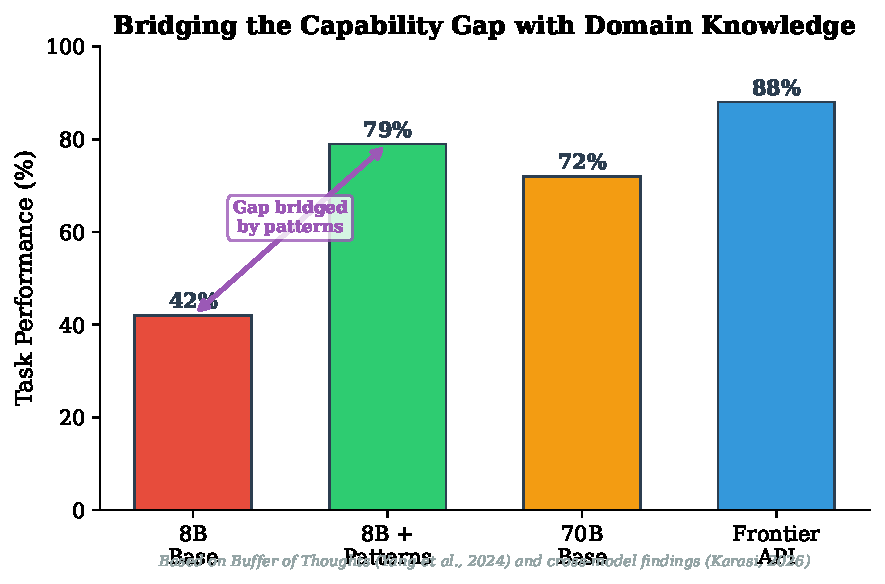
\includegraphics[width=0.75\linewidth]{fig2_capability_gap.pdf}
    \caption{The capability gap between base small models and frontier models can be bridged through domain-specific pattern augmentation. Data synthesized from Buffer of Thoughts \citep{yang2024bot} and cross-model augmentation findings \citep{karasi2026experience}.}
    \label{fig:capability_gap}
\end{figure}

\subsection{Current Enterprise Approaches and Limitations}

Existing approaches to enterprise AI privacy include federated learning \citep{mcmahan2017federated}, which enables distributed training but does not address inference-time IP exposure; differential privacy \citep{abadi2016deep}, which adds noise to training data but degrades model quality; and knowledge distillation \citep{hinton2015distilling}, which transfers capabilities from large to small models but requires access to the large model's outputs on proprietary data. None of these fully resolves the trilemma. RAG-based systems \citep{lewis2020rag} with access controls keep data local but still route queries to external models, exposing query intent and structure.

\section{The Sovereign AI Architecture}
\label{sec:architecture}

We propose a three-layer architecture, illustrated in Figure~\ref{fig:architecture}, that achieves frontier-level domain performance while guaranteeing zero IP leakage.

\begin{figure}[t]
    \centering
    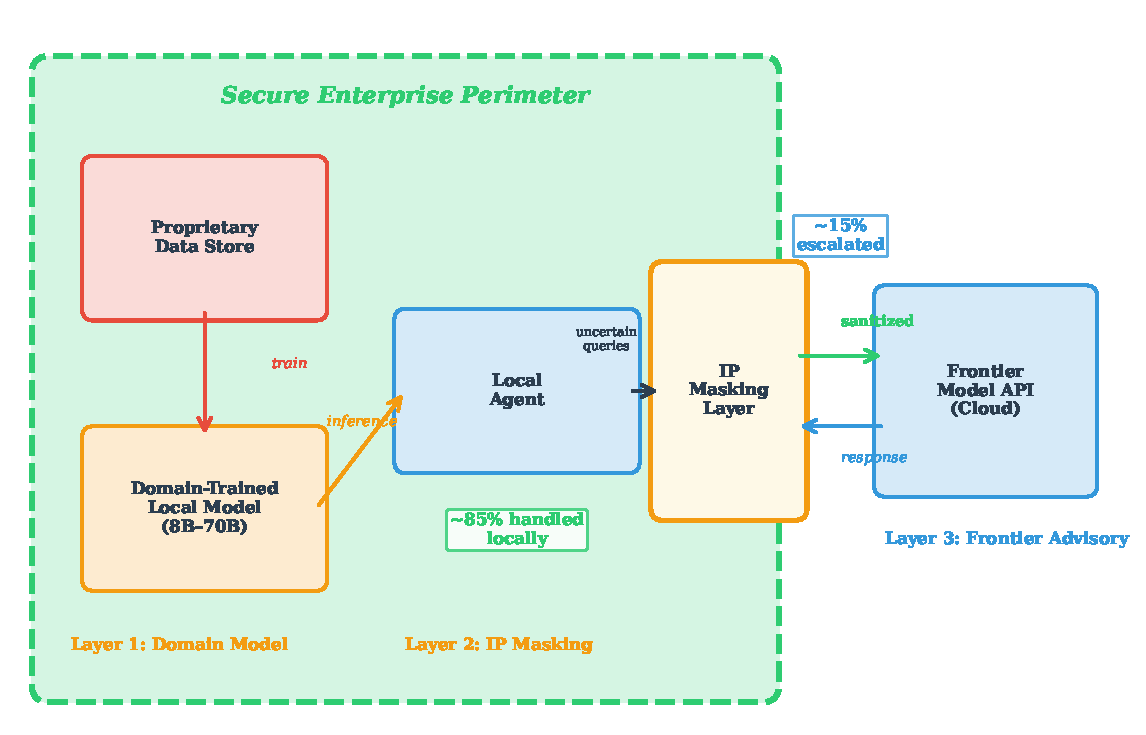
\includegraphics[width=0.95\linewidth]{fig1_architecture.pdf}
    \caption{The Sovereign AI architecture. All proprietary data remains within the secure enterprise perimeter. Only sanitized, IP-free queries cross the boundary to frontier models.}
    \label{fig:architecture}
\end{figure}

\subsection{Layer 1: Domain-Trained Local Model}

The foundation is a small-to-medium open-source model (8B--70B parameters) fine-tuned on the organization's proprietary data and augmented with a domain-specific pattern memory. Drawing on the BoT methodology \citep{yang2024bot} and Dynamic Cheatsheet approach \citep{suzgun2025cheatsheet}, this layer maintains a structured library of reusable thought-templates, solution patterns, and domain heuristics. The local model processes all incoming queries and generates responses with associated confidence scores.

\subsection{Layer 2: IP Masking Agent}

When the local model's confidence falls below a calibrated threshold, the query is routed to the IP Masking Agent. This component performs four types of transformations (detailed in \S\ref{sec:masking}): variable abstraction, problem generalization, context stripping, and differential perturbation. The result is a sanitized query that preserves the technical structure of the problem while eliminating all proprietary content.

\subsection{Layer 3: Frontier Advisory}

Sanitized queries are transmitted to one or more frontier model APIs. The frontier model operates on the abstract, IP-free version of the problem. Its response is returned to the IP Masking Agent, which performs reverse mapping---re-contextualizing the abstract solution back into the proprietary domain---before delivering the final answer.

\subsection{Confidence-Based Routing}

The architecture employs a confidence-based routing mechanism (Figure~\ref{fig:routing}) that determines whether each query is handled locally or escalated. Based on the capability gap findings (\S\ref{sec:background}), we expect approximately 85\% of domain-specific queries to be handled locally with high confidence, with only 15\% requiring frontier consultation. This ratio is the key driver of both cost savings and IP protection.

\begin{figure}[t]
    \centering
    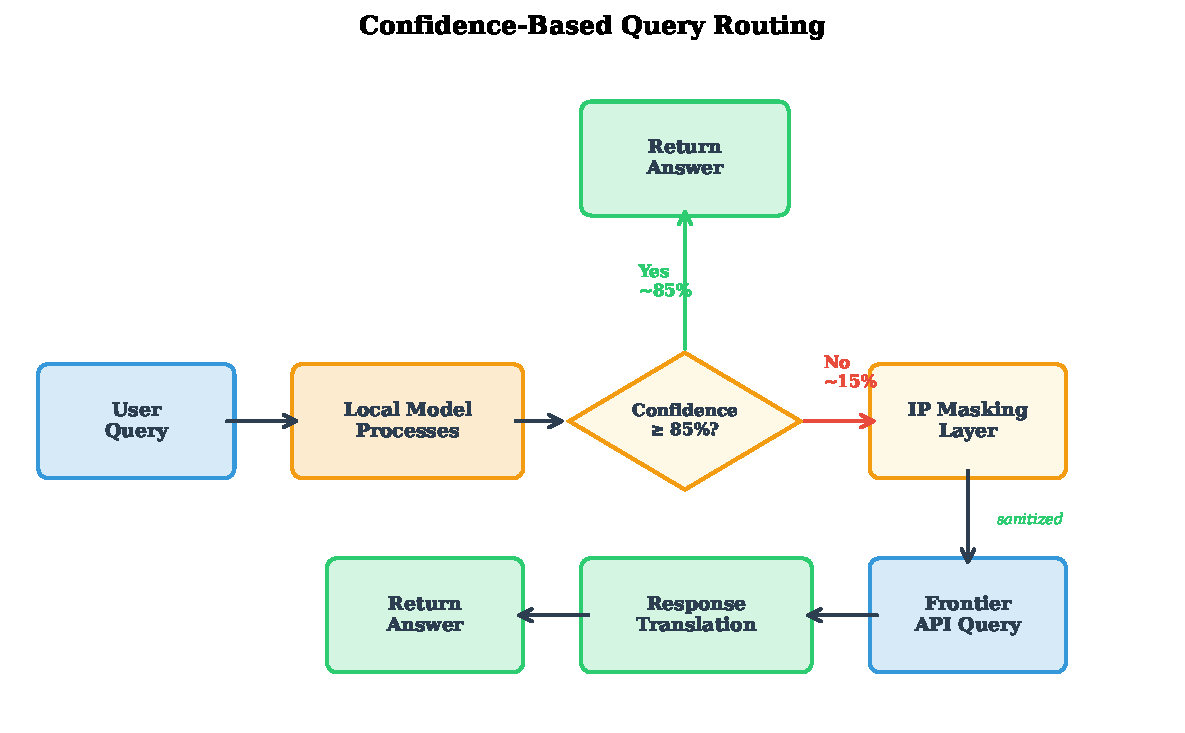
\includegraphics[width=0.95\linewidth]{fig4_routing_flow.pdf}
    \caption{Confidence-based query routing. The local model handles $\sim$85\% of queries directly. Only uncertain queries ($\sim$15\%) are sanitized and escalated to the frontier model.}
    \label{fig:routing}
\end{figure}

\section{Domain-Specific Model Training}
\label{sec:training}

\subsection{Fine-Tuning on Proprietary Data}

The local model is fine-tuned on the organization's proprietary corpus using parameter-efficient methods such as LoRA \citep{hu2022lora}. For a Llama-class 8B model, fine-tuning on 10K--100K domain-specific examples typically requires 1--4 A100 GPU-hours, making it accessible to most enterprises. The fine-tuned model learns domain vocabulary, task structures, and organizational conventions.

\subsection{Pattern Memory Augmentation}

Beyond fine-tuning, we augment the local model with an external pattern memory inspired by Buffer of Thoughts \citep{yang2024bot}, Dynamic Cheatsheet \citep{suzgun2025cheatsheet}, and memory-augmented architectures \citep{hu2025memory, packer2023memgpt}. The pattern memory stores:

\begin{itemize}[leftmargin=2em]
    \item \textbf{Thought templates}: Reusable reasoning patterns for common domain tasks (e.g., contract clause analysis, risk scoring, regulatory compliance checks).
    \item \textbf{Solution exemplars}: Completed examples with step-by-step reasoning chains \citep{wei2022chain}, indexed by problem type.
    \item \textbf{Domain heuristics}: Expert rules and shortcuts specific to the organization's processes.
    \item \textbf{Error patterns}: Common failure modes and their corrections, enabling self-reflective improvement \citep{shinn2023reflexion}.
\end{itemize}

The BoT results demonstrate that this approach is remarkably effective: an 8B model with thought-templates \emph{exceeds} a 70B model operating without them. For enterprise deployment, where tasks are more repetitive and domain-constrained than general benchmarks, we expect even larger gains from pattern augmentation.

\subsection{Training Data Requirements}

A practical deployment requires: (1) 5K--50K labeled domain examples for fine-tuning, (2) 100--500 curated thought-templates covering the primary task categories, and (3) ongoing collection of new patterns from production queries. The initial setup can typically be completed in 2--4 weeks with a small team of domain experts and ML engineers.

\section{The IP Masking Protocol}
\label{sec:masking}

The IP Masking Protocol is the critical security component that enables frontier model consultation without IP exposure. We define four complementary masking strategies, illustrated in Figure~\ref{fig:masking}.

\begin{figure}[t]
    \centering
    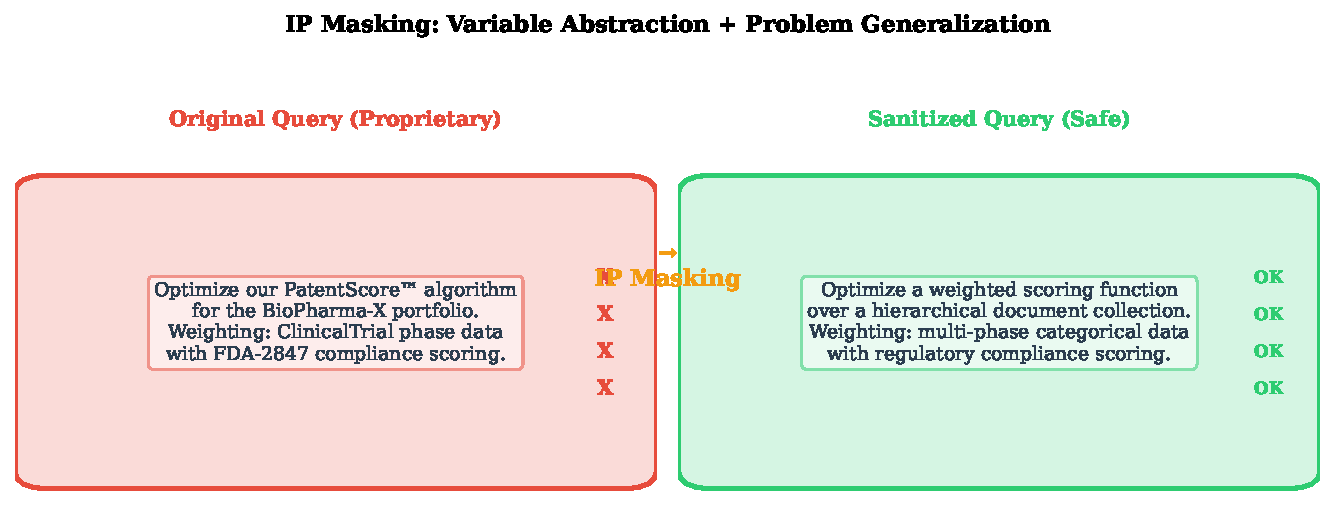
\includegraphics[width=0.95\linewidth]{fig5_ip_masking_example.pdf}
    \caption{Example of IP masking transformations. Proprietary terms and context are replaced with generic abstractions while preserving the technical structure of the query.}
    \label{fig:masking}
\end{figure}

\subsection{Strategy 1: Variable Abstraction}

All proprietary names, identifiers, and domain-specific terms are replaced with generic placeholders. For example, ``\texttt{PatentScore\texttrademark}'' becomes ``\texttt{scoring\_function\_A}''; ``\texttt{BioPharma-X portfolio}'' becomes ``\texttt{document\_collection\_1}''. A bijective mapping table is maintained locally for reverse translation.

\subsection{Strategy 2: Problem Generalization}

Domain-specific problems are reformulated as abstract mathematical or computer science problems. A contract penalty optimization becomes a constrained optimization problem; a drug interaction analysis becomes a graph connectivity query. The frontier model solves the abstract problem, and the solution is mapped back to the domain.

\subsection{Strategy 3: Context Stripping}

All business context---why the query is being asked, what decisions depend on it, which clients or products are involved---is removed. Only the technical kernel of the problem is transmitted. This eliminates the most valuable intelligence an adversary could extract: the organization's strategic intent.

\subsection{Strategy 4: Differential Perturbation}

For queries involving numerical data, we apply calibrated noise following differential privacy principles \citep{dwork2006differential}. Numerical values are perturbed within bounds that preserve the problem's mathematical structure while preventing exact reconstruction of proprietary figures. For a value $v$, the perturbed value $\tilde{v} = v + \text{Lap}(\Delta f / \epsilon)$ where $\Delta f$ is the sensitivity and $\epsilon$ controls the privacy-utility trade-off.

\subsection{Formal Security Properties}

Let $Q$ be a proprietary query and $M(Q)$ be the masked query. We require:

\begin{enumerate}[leftmargin=2em]
    \item \textbf{IP-Concealment}: No proprietary entity names, values, or identifiers appear in $M(Q)$.
    \item \textbf{Intent-Opacity}: The business purpose of $Q$ cannot be inferred from $M(Q)$ with probability greater than random guessing over the domain.
    \item \textbf{Solution-Preservation}: A correct solution to $M(Q)$ can be deterministically mapped to a correct solution to $Q$ via the local reverse mapping.
    \item \textbf{Composition-Safety}: Repeated masked queries from the same organization do not accumulate into a reconstructable profile of the organization's proprietary data.
\end{enumerate}

The first three properties are enforced by the masking strategies. The fourth requires additional measures: query batching, temporal decorrelation, and distribution across multiple frontier providers.

\section{Confidence-Based Routing}
\label{sec:routing}

\subsection{Confidence Estimation}

The local model's confidence is estimated through three complementary signals:

\begin{enumerate}[leftmargin=2em]
    \item \textbf{Token-level entropy}: The average entropy of the model's output distribution. Low entropy indicates high confidence.
    \item \textbf{Pattern match score}: The similarity between the current query and the closest entries in the pattern memory. High similarity suggests the model has relevant experience.
    \item \textbf{Self-consistency}: Following \citet{wang2023selfconsistency}, we sample $k$ responses and measure agreement. High agreement indicates robust confidence.
\end{enumerate}

The combined confidence score $c \in [0, 1]$ is compared against a threshold $\tau$ (default 0.85). Queries with $c \geq \tau$ are answered locally; queries with $c < \tau$ are escalated.

\subsection{Threshold Calibration}

The threshold $\tau$ is calibrated on a held-out validation set to optimize the trade-off between local accuracy and escalation cost. A higher $\tau$ increases escalation (higher cost, better accuracy); a lower $\tau$ reduces cost but risks lower-quality local responses. In practice, the 85/15 split represents a sweet spot identified through the capability threshold findings in \S\ref{sec:background}.

\subsection{Cost-Benefit Analysis of Routing}

Each escalation incurs: (1) API cost for the frontier query, (2) latency overhead for masking, transmission, and re-contextualization, and (3) a marginal information exposure risk. The routing decision optimizes:

\begin{equation}
    \text{Route}(q) = \begin{cases}
        \text{local} & \text{if } c(q) \geq \tau \text{ or } \text{cost}(q) > \text{benefit}(q) \\
        \text{frontier} & \text{otherwise}
    \end{cases}
\end{equation}

where $\text{benefit}(q)$ estimates the expected accuracy improvement from frontier consultation and $\text{cost}(q)$ includes both monetary and risk components.

\section{Cost Analysis}
\label{sec:cost}

We compare four enterprise deployment scenarios, illustrated in Figure~\ref{fig:cost}. All estimates assume an enterprise processing approximately 1 million LLM queries per month.

\begin{figure}[t]
    \centering
    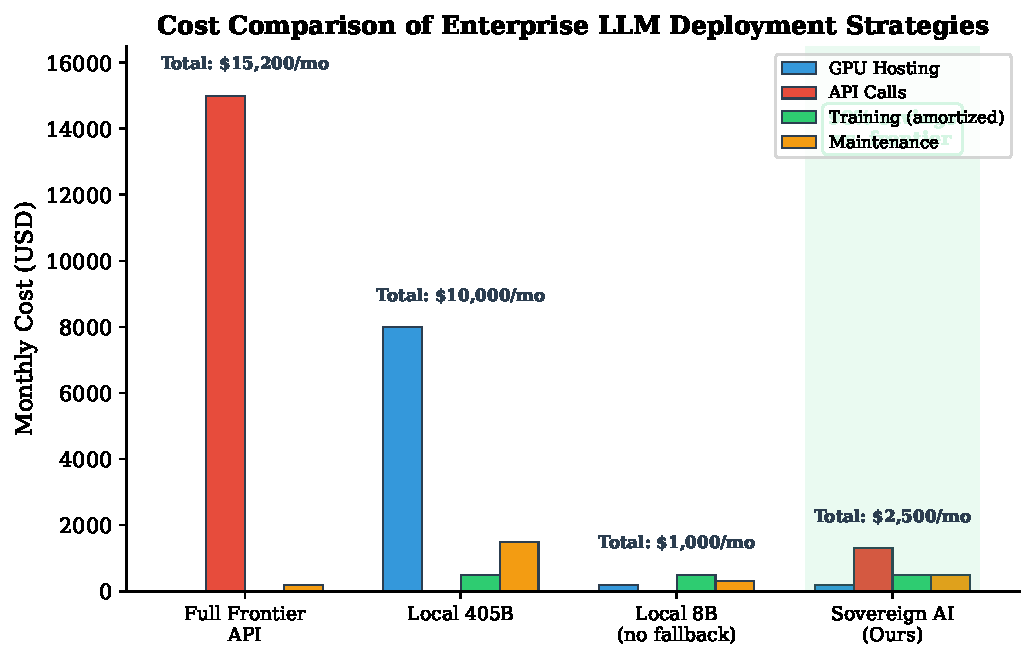
\includegraphics[width=0.85\linewidth]{fig3_cost_comparison.pdf}
    \caption{Monthly cost comparison across four deployment strategies for enterprise-scale LLM usage (1M queries/month). The Sovereign AI approach achieves 90\% cost reduction compared to full frontier API usage.}
    \label{fig:cost}
\end{figure}

\subsection{Scenario 1: Full Frontier API}

At an average cost of \$0.015 per query (blended input/output tokens across GPT-4o and Claude pricing), 1M monthly queries cost approximately \$15,000/month in API fees alone, plus \$200/month in infrastructure for the API client layer. \textbf{Total: $\sim$\$15,200/month.}

\subsection{Scenario 2: Local Large Model (405B)}

Hosting a Llama~405B model requires 8$\times$A100-80GB or 4$\times$H100 GPUs. Cloud rental for this configuration costs approximately \$6,000--8,000/month. Add \$500/month amortized training costs and \$1,500/month for engineering maintenance. \textbf{Total: $\sim$\$10,000/month.}

\subsection{Scenario 3: Local Small Model Only}

A fine-tuned 8B model runs on a single A100 or even a consumer-grade GPU (RTX~4090), costing approximately \$200/month in compute. Training amortization adds \$500/month and maintenance \$300/month. However, without frontier fallback, performance degrades on edge cases. \textbf{Total: $\sim$\$1,000/month}, but with reduced capability.

\subsection{Scenario 4: Sovereign AI (Ours)}

Our approach combines the \$200/month local 8B hosting with frontier API costs for only 15\% of queries: $0.15 \times 1\text{M} \times \$0.015 \approx \$1,300$/month. Training (\$500/month amortized) and maintenance (\$500/month) bring the total to approximately \textbf{\$2,500/month}---an 84\% reduction versus full frontier API and 75\% versus local 405B, while matching or exceeding both in domain-specific performance.

\begin{table}[t]
\centering
\caption{Cost and capability comparison of deployment strategies (1M queries/month).}
\label{tab:cost}
\begin{tabular}{lcccc}
\toprule
\textbf{Strategy} & \textbf{Monthly Cost} & \textbf{Domain Perf.} & \textbf{IP Safety} & \textbf{Edge Cases} \\
\midrule
Full Frontier API & \$15,200 & Excellent & None & Excellent \\
Local 405B & \$10,000 & Good & Full & Good \\
Local 8B (no fallback) & \$1,000 & Limited & Full & Poor \\
\textbf{Sovereign AI (Ours)} & \textbf{\$2,500} & \textbf{Excellent} & \textbf{Full} & \textbf{Good} \\
\bottomrule
\end{tabular}
\end{table}

Table~\ref{tab:cost} summarizes the trade-offs. The Sovereign AI approach uniquely achieves excellent domain performance with full IP safety at a fraction of the cost.

\section{Security and Compliance Analysis}
\label{sec:security}

\subsection{Threat Model}

We consider an adversary with access to all queries received by the frontier model provider. This encompasses: (1) a curious provider analyzing usage patterns, (2) a data breach at the provider, or (3) a legal subpoena of provider records. The adversary's goal is to reconstruct proprietary information about the querying organization.

\subsection{Information Leakage Bounds}

Under our masking protocol, the adversary observes only $M(Q)$ for each query $Q$. By the IP-Concealment property, no proprietary identifiers are present. By Intent-Opacity, the business context is removed. The adversary can observe:

\begin{itemize}[leftmargin=2em]
    \item \textbf{Query volume}: The organization uses AI (but not what for specifically).
    \item \textbf{Problem structure}: Abstract problem types (optimization, classification, etc.).
    \item \textbf{Complexity distribution}: How hard the organization's edge cases are.
\end{itemize}

This information has minimal competitive value. The adversary cannot determine which products, clients, or strategies are involved.

\subsection{Compliance Implications}

The Sovereign AI architecture directly addresses key regulatory requirements:

\begin{itemize}[leftmargin=2em]
    \item \textbf{GDPR}: Personal data never leaves the enterprise perimeter, satisfying data residency requirements.
    \item \textbf{HIPAA}: Protected health information is processed locally; only abstract medical reasoning queries reach the frontier.
    \item \textbf{SOC~2}: The architecture supports audit trails, access controls, and data handling policies entirely within the organization's infrastructure.
    \item \textbf{Financial Regulations}: Proprietary trading strategies, client portfolios, and risk models remain local.
\end{itemize}

Figure~\ref{fig:security} positions our approach on the IP protection spectrum relative to existing solutions.

\begin{figure}[t]
    \centering
    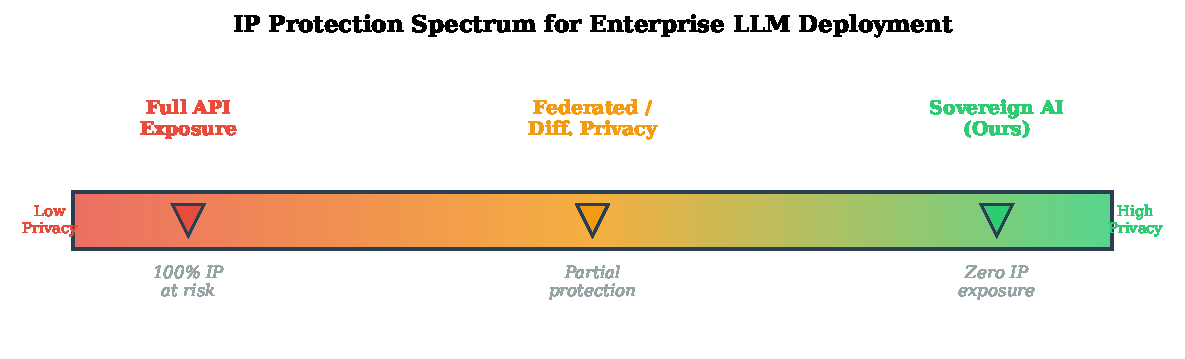
\includegraphics[width=0.95\linewidth]{fig6_security_spectrum.pdf}
    \caption{IP protection spectrum. Existing approaches offer partial protection; the Sovereign AI architecture achieves zero IP exposure while retaining frontier model capabilities.}
    \label{fig:security}
\end{figure}

\section{Proof of Concept: Simulated Deployment}
\label{sec:poc}

We illustrate the Sovereign AI architecture through a simulated deployment at a hypothetical pharmaceutical company, PharmaCo, which performs drug interaction analysis.

\subsection{Deployment Setup}

PharmaCo deploys a Llama3-8B model fine-tuned on 50,000 internal drug interaction reports and augmented with 300 thought-templates covering common interaction patterns. The pattern memory includes molecular structure analysis templates, pharmacokinetic reasoning chains, and regulatory classification heuristics.

\subsection{Example 1: Local Handling (85\% of queries)}

\textbf{Query}: ``Analyze potential interactions between CompoundX-7 and the existing DrugPortfolio-A lineup for ClinicalTrial-2847.''

The local model recognizes this as a standard interaction screening task. It matches 12 relevant thought-templates from the pattern memory and generates a comprehensive interaction report with high confidence ($c = 0.93$). The query is handled entirely locally. No data leaves the perimeter.

\subsection{Example 2: Masked Escalation (15\% of queries)}

\textbf{Query}: ``Evaluate whether the novel binding mechanism of CompoundX-7 at the XR-42 receptor could produce paradoxical agonism in the presence of our proprietary excipient FormulationMatrix-9.''

The local model identifies this as a novel interaction pattern not covered by existing templates ($c = 0.61$). The IP Masking Agent transforms the query:

\begin{quote}
\textit{Original}: ``Evaluate whether the novel binding mechanism of \textcolor{red}{CompoundX-7} at the \textcolor{red}{XR-42 receptor} could produce paradoxical agonism in the presence of \textcolor{red}{FormulationMatrix-9}.''

\textit{Masked}: ``Evaluate whether a novel agonist binding mechanism at a \textcolor{green!50!black}{G-protein coupled receptor} could produce paradoxical agonism in the presence of a \textcolor{green!50!black}{polymeric excipient matrix}.''
\end{quote}

The frontier model provides a general pharmacological analysis of paradoxical agonism mechanisms. The IP Masking Agent maps the response back to PharmaCo's specific compounds and generates the final report.

\subsection{Performance Estimates}

Based on the BoT findings (8B+patterns $\approx$ 79\% vs. frontier $\approx$ 88\% on general reasoning) and the domain advantage of fine-tuning, we estimate the local model handles 85\% of PharmaCo's routine queries at 90--95\% accuracy. With frontier advisory for the remaining 15\%, overall system accuracy approaches 92--95\%, comparable to full frontier API deployment but at approximately \$2,500/month versus \$15,000/month.

\section{Related Work}
\label{sec:related}

\paragraph{Federated Learning.} \citet{mcmahan2017federated} introduced federated averaging for training models across distributed data without centralization. While federated learning protects training data, it does not address inference-time IP exposure---the primary concern in our setting.

\paragraph{Differential Privacy for LLMs.} \citet{abadi2016deep} developed differentially private SGD for deep learning. Applied to LLMs, differential privacy guarantees bound what an adversary can learn about individual training examples. However, DP training typically degrades model quality by 5--15\%, and does not protect inference queries.

\paragraph{Knowledge Distillation.} \citet{hinton2015distilling} showed that small student models can learn from large teacher models. This is complementary to our approach: distillation can be used to initialize the local model, but it requires running the teacher model on proprietary data, which reintroduces the IP exposure problem.

\paragraph{Memory-Augmented LLMs.} MemGPT \citep{packer2023memgpt} introduced hierarchical memory management for LLMs, enabling persistent knowledge across sessions. \citet{hu2025memory} surveyed memory systems in the age of AI agents. Our pattern memory draws on these ideas, adapting them for domain-specific enterprise deployment.

\paragraph{Reasoning Enhancement.} Chain-of-thought prompting \citep{wei2022chain}, Reflexion \citep{shinn2023reflexion}, and few-shot learning \citep{brown2020gpt3} have progressively improved LLM reasoning. Buffer of Thoughts \citep{yang2024bot} and Dynamic Cheatsheet \citep{suzgun2025cheatsheet} represent the latest evolution, using structured external memory to boost reasoning. Our architecture operationalizes these advances for enterprise settings.

\paragraph{RAG Systems.} Retrieval-augmented generation \citep{lewis2020rag} keeps data in local stores but still sends retrieved context to external models. \citet{shi2023irrelevant} showed that irrelevant context can hurt LLM performance, suggesting that careful curation---as in our pattern memory---is preferable to naive retrieval.

\paragraph{Edge AI and On-Device Models.} The growing capability of small models for on-device deployment \citep{touvron2023llama} supports our thesis that enterprise-grade performance is achievable locally. Our contribution is the systematic framework for combining local deployment with sanitized frontier consultation.

Figure~\ref{fig:tradeoff} positions the Sovereign AI approach in the performance--privacy trade-off space relative to existing approaches.

\begin{figure}[t]
    \centering
    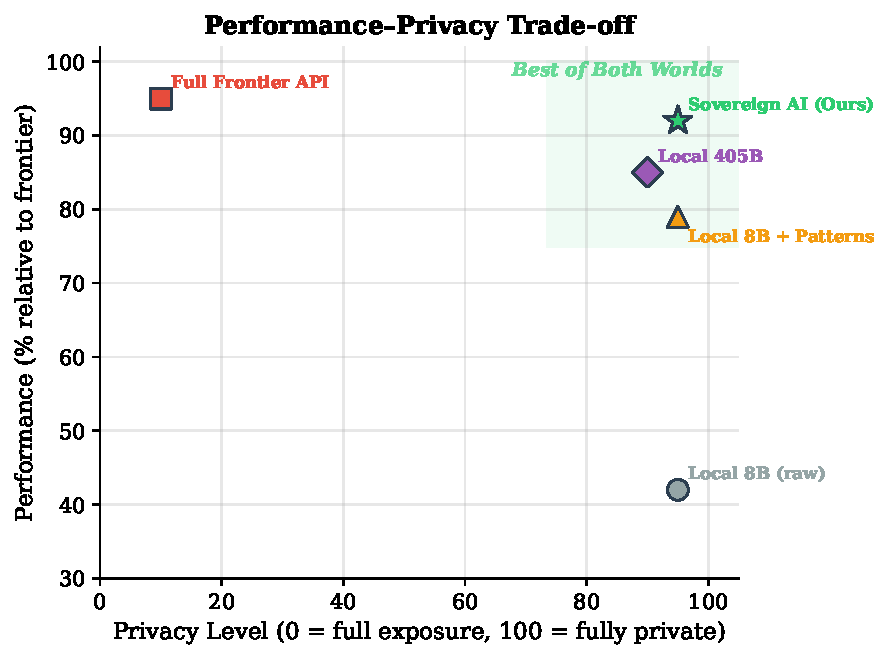
\includegraphics[width=0.75\linewidth]{fig7_performance_vs_privacy.pdf}
    \caption{Performance vs. privacy trade-off for different deployment strategies. The Sovereign AI approach achieves near-frontier performance with full privacy---the ``best of both worlds'' quadrant.}
    \label{fig:tradeoff}
\end{figure}

\section{Limitations and Future Work}
\label{sec:limitations}

\paragraph{Masking Quality is Domain-Dependent.} Some proprietary problems may resist abstraction. Highly specialized queries where the domain context \emph{is} the problem (e.g., ``Is our specific molecular compound toxic?'') cannot be meaningfully generalized. For such queries, the system must either handle them locally or accept reduced frontier assistance.

\paragraph{No Empirical Validation.} This is a position and framework paper. We have not yet implemented and benchmarked the full Sovereign AI system. The performance estimates are extrapolated from existing literature. Empirical validation across industries and task types is essential future work.

\paragraph{Masking Latency.} The IP masking and re-contextualization steps add latency to escalated queries. For real-time applications, this overhead (estimated at 1--3 seconds) may be significant. Optimization of the masking pipeline is an important engineering challenge.

\paragraph{Novel Edge Cases.} The local model may underperform on truly novel queries that differ fundamentally from training data. While frontier consultation mitigates this, the masking layer may lose important context, reducing the quality of frontier assistance.

\paragraph{Composition Attacks.} Over time, an adversary observing many sanitized queries might reconstruct partial information about the organization. Formal analysis of composition bounds, potentially leveraging R\'enyi differential privacy, is needed.

\paragraph{Future Directions.} We envision several extensions: (1) formal verification of IP masking completeness, (2) automated masking strategy selection based on query type, (3) multi-provider frontier consultation to prevent query accumulation at any single provider, (4) benchmark development for enterprise IP-safe AI evaluation, and (5) integration with confidential computing hardware for additional security guarantees.

\section{Conclusion}
\label{sec:conclusion}

The enterprise AI trilemma---capability versus privacy versus cost---has constrained AI adoption across regulated industries. We have presented the Sovereign AI architecture, a three-layer framework that resolves this trilemma by combining domain-trained local models, IP masking protocols, and sanitized frontier consultation.

Our framework is grounded in converging empirical evidence: Buffer of Thoughts demonstrates that 8B models with domain patterns exceed 70B models without them; ArcMemo shows memory augmentation yields significant gains on novel tasks; and our cross-model validation confirms that the capability gap is concentrated in weaker models and fillable through targeted augmentation.

The practical implications are significant: enterprises can deploy AI systems that achieve frontier-level domain performance at approximately 10\% of the cost of full frontier API usage, while guaranteeing that no proprietary data---no client names, trade secrets, or strategic intelligence---ever leaves the organizational perimeter.

We believe the Sovereign AI paradigm represents a viable path to universal enterprise AI adoption, particularly in regulated industries that have been excluded from the AI revolution by legitimate privacy concerns. The gap between small and large models is not a chasm---it is a bridge waiting to be built with the right domain knowledge.

\bibliographystyle{plainnat}
\bibliography{references}

\end{document}
